\documentclass[letterpaper,journal]{IEEEtran}
\usepackage[T1]{fontenc}
\usepackage[utf8]{inputenc}
\usepackage{amsmath,amssymb,graphicx,booktabs,array,tabularx,ragged2e,textcomp,url,xurl,cite,stfloats,placeins}
\usepackage[hidelinks]{hyperref}
\graphicspath{{../figs/}}
\urlstyle{same}
\providecommand{\tightlist}{\setlength{\itemsep}{0pt}\setlength{\parskip}{0pt}}
\setlength{\emergencystretch}{1.5em}
\hyphenation{rein-force-ment en-vi-ron-ment accel-er-a-tion}
\pagestyle{plain}

\begin{document}
\title{Environment-Aware Reinforcement Learning for Electric Vehicle Eco-Driving with Smooth Execution}
\author{Ziran Peng and Zeyu Fan\thanks{Ziran Peng and Zeyu Fan are with the School of Transportation and Electrical Engineering, Hunan University of Technology, Zhuzhou, China (e-mail: pengziran@hut.edu.cn; m24085800005@stu.hut.edu.cn). Corresponding author: Ziran Peng.}}
\maketitle
\begin{abstract}Environment-aware electric vehicle control requires visual evidence to produce useful commands and smooth motion. Command regularization alone cannot preserve braking-release feasibility or accommodate changes in perceived stopping targets. This paper develops a camera-to-control interface, a release-aware execution algorithm, and a discrete preparation reference. Frozen event detection supplies road-target memory, while a separately supervised representation supports a twin delayed deep deterministic policy gradient controller. The executor combines a sampled release bound with target-distance backup checks. A target-update identity separates physical propagation from memory revision; a two-stage linear program distinguishes feasible preparation from cost-free preparation. On a synthetic 4 km development route, the visual configuration completes 27/27 evaluations without recorded signal or curve-speed violations. A separate frozen-actor comparison reduces cumulative squared jerk by 26.50\%, with 0.11 s additional mean travel time. Record-based diagnosis separates 195 stopping-branch events into 163 noncreeping events and 32 small propagation discrepancies without jerk-limit exceedance. Inward target updates exhaust positive propagated margins in 159/163 noncreeping cases. Complete memory replay reproduces 12,081 recorded states; an experimental update guard restores the static backup margin in two of three selected visual cases, without establishing a driving benefit. A locally installable environment companion exposes the command, perception, execution, and logging interfaces. These results support evaluating perception through its control targets alongside completed travel, energy, and realized smoothness.\end{abstract}
\begin{IEEEkeywords}Electric vehicles, eco-driving, energy efficiency, environment-aware reinforcement learning, visual perception, smooth execution\end{IEEEkeywords}
\section{Introduction}

An electric vehicle approaching a signal needs correct information while useful stopping or passing options remain. Preparing for every uncertain signal can preserve stopping capability but waste time and energy on passing branches. Conversely, a gradually changing command can still cause abrupt braking release near a target.

These difficulties connect perception, learning, and execution. Images provide intermittent evidence, RL proposes a command, and the executor reconciles it with dynamics and traffic targets. Assessment must therefore measure completed travel and violations alongside energy, time, and actual jerk.

The three questions studied here are whether camera-derived targets support compliant driving, how to preserve a smooth brake-and-release response, and what progress cost is necessary before stop-or-pass uncertainty is resolved. A conservative target can exclude a smooth response even while the vehicle can still stop before the physical line. We examine this distinction through explicit execution checks, recorded target updates, and a separate preparation reference. The components share a control interface without assuming an optimal learned policy.

The contributions are as follows.

\textbf{C1 --- A camera-to-control interface with localized operating outcomes.} Camera-derived event memory and a supervised policy representation support visual driving. The interface separates detection, color adoption, target revision, and execution, permitting completed travel and compliance to be assessed alongside the location and context of each observed override.

\textbf{C2 --- A release-aware execution algorithm for comfort-oriented commands.} An explicit sampled release bound and target-distance backups retain candidate actions before selecting the one nearest the policy preference. A target-update relation, trigger-aligned accounting, and memory replay distinguish propagation discrepancies from changes that exhaust a retained response. Frozen-actor comparisons quantify the complete executor's smoothness effect.

\textbf{C3 --- A discrete preparation reference for rule assessment.} A two-stage linear program (LP) distinguishes common feasibility from cost-free preparation under sampled vehicle bounds. Complete delay scans and lower-grid references at actual adoption times compare preparation rules with modeled progress costs. A closed-form maneuver proposition supplies an explanatory special case.

\section{Related Work}

Eco-driving optimizes energy and travel time using traffic and road information. Dynamic programming and look-ahead methods address signal coordination and long horizons \cite{R-DP1}, \cite{R-DP2}, including road curvature \cite{R-CURV}. RL studies address traffic uncertainty and learned driving decisions \cite{R-RL1}, \cite{R-RL2}, \cite{R-RL3}; IntersectionZoo provides a broader contextual benchmark \cite{R-IZOO}. The present work contributes a single-vehicle visual and execution assessment on declared development routes. The structured 20 km results provide a separate long-route reference for these interface studies.

TD3 reduces function-approximation error through twin critics, delayed policy updates, and target-policy smoothing \cite{R-TD3}. Its target noise is not a temporal constraint on vehicle acceleration. CAPS regularizes policies for smooth control \cite{R-CAPS}, while jerk-limited trajectory generation explicitly constrains motion \cite{R-RUCKIG}. Predictive safety filters modify learned commands using future constraint satisfaction \cite{R-PSF}, and backup control barrier functions construct admissible behavior from a specified backup policy \cite{R-BCBF}. These establish the general rationale for filtering a preferred action. The present specialization makes the sampled release bound and target-distance search explicit, then examines how perceived target revisions alter that search. It evaluates a complete longitudinal executor; it does not introduce a new general filtering or safety principle.

Action projection can map distinct commands to the same applied action and affect learning gradients \cite{R-PROJ}. This is directly relevant when one command is held over several execution updates. The learning interface is therefore reported separately from the fixed-policy driving outcomes. Action-sufficient representations \cite{R-ASR} and value-equivalent modeling \cite{R-VE} motivate retaining decision-relevant information, but camera-driven task completion alone does not establish representation sufficiency or a novel joint-learning rule.

Preview control already links anticipation to actuator rate constraints \cite{R-PREVIEW}. The preparation analysis here distinguishes preserving a common stop-or-pass response from preserving it without progress loss. The discrete LP is the primary reference at vehicle parameters; a restricted continuous maneuver family supplies a closed-form explanation. The shared object is the response retained under a target and an execution bound. This links camera-derived target quality, smooth command realization, and preparation cost while preserving the distinct information conditions of each comparison.

\section{System And Comparison Protocols}

\subsection{Protocols and vehicle objective}

\begin{table*}[!t]
\centering
\renewcommand{\thetable}{I}
\caption{Information and intervention protocols. Each row defines its own comparison and denominator. The information supplied to the actor and executor is specified separately.}
\setlength{\tabcolsep}{3pt}
\renewcommand{\arraystretch}{1.12}
\begin{tabularx}{\textwidth}{@{}>{\hsize=0.680000\hsize\linewidth=\hsize\raggedright\arraybackslash}X>{\hsize=1.280000\hsize\linewidth=\hsize\raggedright\arraybackslash}X>{\hsize=1.320000\hsize\linewidth=\hsize\raggedright\arraybackslash}X>{\hsize=0.720000\hsize\linewidth=\hsize\raggedright\arraybackslash}X@{}}
\toprule
\textbf{Protocol} & \textbf{Policy and information} & \textbf{Execution or intervention} & \textbf{Role} \\
\midrule
P-V: visual 4 km & F/S, three seeds and nine conditions; camera memory and image representation & Perceived targets; release-aware base; no true-position terminal command override & Visual system operation \\
P-C: comfort & Fixed A/B from one seed; structured road events and phase timing & Original versus complete executor; nine conditions per actor & Combined executor effect \\
P-T: timing use & Fixed A; actor receives SPaT in both arms & Executor current color versus color plus countdown; nine pairs & Timing-use intervention \\
P-B: short branches & Constant command and three frozen S policies; two approach states & Output-gated color; early or two preparation rules; jerk 2/3/4 & Preparation response and cost \\
P-LP: reference & No actor; known line; fixed-time scene revelation & Shared acceleration prefix; explicit stop/pass constraints & Within-model feasibility and cost \\
Reference context & Eight 20 km structured-input seeds; separate constant-command visual probe & Original archived protocols & Context and claim calibration \\
\bottomrule\end{tabularx}
\end{table*}

The 4 km route contains a 35 km/h curve at 1450--1550 m and a signal at 3000 m. Nine conditions cross three pack states and signal offsets 0, 30, and 60 s; initial speed is 16 m/s. Green lasts 30 s in a 90 s cycle, and other phases are nonpassable. Short-route tasks retain their 600 s limit and 480 s clock normalization. Historical 20 km runs retain the 1312.5 s task deadline.

The vehicle model uses a 1928 kg mass and Leaf Plus-based road load \cite{S4}. A separately parameterized 35040 Wh NMC pack models SOC- and temperature-dependent charge acceptance. Traction, regeneration, and rejected demand allocated to friction braking are engineering approximations; complete assumptions appear in Supplementary Section A \cite{S3}, \cite{S5}. Recorded reward combines continuous energy and time costs with overspeed and event charges:

\[\begin{aligned}
r_k={}&-P_{b,k}\delta/E_0-\lambda_T\delta\\
&-k_{\rm os}\min\{(v_k-v_{\max,k})_+,5\}^2\delta,\\
R={}&-0.036E_{\rm Wh}-0.08T-P,
\end{aligned}\tag{1}\]

where \(\delta=0.5\) s, \(E_0=100\) kJ, \(\lambda_T=0.08\) s\(^{-1}\), \(k_{\rm os}=0.02\), and \(P\) collects recorded event and unfinished-trip penalties. Completion and violations use all attempts. Completed-trip cost contrasts state their condition sets; failure-shortened energy is not counted as a saving.

\subsection{Commands and applied motion}

Let \(n\) index policy decisions and \(k\) index physical substeps. The normalized command \(u_n\) is held for four substeps, while perception, memory, and execution can update at every substep. With physical state \(s_k\), event memory \(M_k\), additional executor state \(\mu_k\), and protocol \(\nu\),

\[\begin{aligned}
c(u)&=\begin{cases}2.6u,&u\ge0,\\3.5u,&u<0,\end{cases}\\
a_{k+1}&=\mathcal E_\nu(s_k,M_k,\mu_k,c(u_n)),\\
v_{k+1}&=v_k+\delta a_{k+1},\\
x_{k+1}&=x_k+\tfrac{\delta}{2}(v_k+v_{k+1}).
\end{aligned}\tag{2}\]

Equation (2) gives nominal constant-acceleration integration; boundary handling and emergency fallback are recorded separately. A held command and its first applied acceleration are distinct: identical first substeps can be followed by different later motion. The retained policy input is not assumed to contain every executor memory field.

\subsection{Camera-derived events and the policy representation}

The visual system renders \(96\times160\) RGB frames at 2 Hz. A warning sign announces a curve 400 m ahead with fixed 35 km/h semantics; an exit sign releases that limit. Lamps appear within 200 m, without a displayed countdown. Runtime road-event targets come from perception and memory rather than a map or SPaT oracle. The route-specific sign conventions remain part of this synthetic environment.

Two separate image-processing instances serve different control functions:

\[\begin{aligned}
\zeta_k&=D_\psi(I_k),\\
M_k&=\mathcal F(M_{k-1},\zeta_k,\text{ego motion}),\\
z_n&=E_\theta(I_{k_n-3:k_n},\mathrm{valid},\mathrm{age}),\\
y_n&=[q_n(M_{k_n}),z_n,\mathrm{meta}_n].
\end{aligned}\tag{3}\]

The frozen event detector \(D_\psi\) predicts event identity, range, and color; memory propagates range with ego motion and applies freshness, voting, and commitment rules. The separate encoder produces a 64-dimensional \(Z\). The 87 policy inputs comprise 13 legacy-format vehicle/memory/clock fields, 64 representation components, four metadata fields, and six additional memory fields. Predicted ROI pooling supports a separate color-supervision head; it is not an input dependency of the delivered \(Z\) path.

\begin{figure*}[!t]
\centering
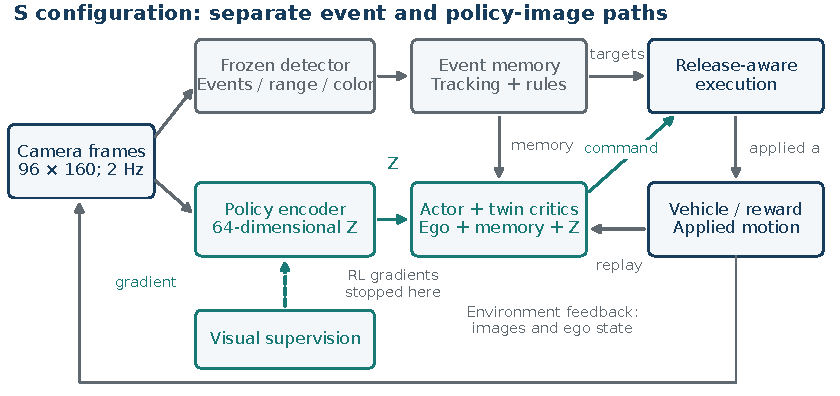
\includegraphics[width=\textwidth]{fig1_interfaces.pdf}
\renewcommand{\thefigure}{1}
\caption{Camera-to-control architecture for S. Frozen detection supplies event memory and execution targets; a separate encoder supplies the policy representation. Visual supervision updates that encoder, while actor/critic RL updates use detached features. Vehicle transitions train the policy and critics; they do not update the frozen event detector. The jerk preference and release-aware execution act at different points in this chain.}
\end{figure*}

F freezes the policy encoder; S trains it through visual supervision, including a color head on \(Z\). For the encoder gradients supplied to Adam,

\[g_{\theta,F}=0,\qquad g_{\theta,S}=\lambda_v\nabla_\theta\mathcal L_{\rm vis}.\tag{4}\]

Actor gradients stop at the encoder in every archived arm. J adds critic feedback, and JH restricts it to temporal fusion; both are supplementary diagnostics. The learner has a known action-semantic limitation: critic regression uses a first-applied-action label while bootstrapping queries a raw target command. Together with omitted executor memory, this prevents interpreting the runs as validation of a new TD3 learning rule. Supplementary Section B gives the complete supervised loss, implemented objectives, and gradient paths. The reported driving outcomes evaluate these archived fixed policies.

Seeds 7/8/9 use camera seeds 77/78/79, one detector and supervised pool, 2400 common adaptation substeps, and approximately 9000 further substeps per arm. Evaluation matches per-condition camera streams, with trajectory-dependent images. All arms share the comfort coefficient. S is selected on development completion, without an untouched confirmation set.

The P-V base executor is byte-identical to the release-aware base used in P-C. Visual policies and that base have therefore already operated together. Perceived targets, wrappers, and phase information differ across protocols, so this identity does not identify individual execution-feature effects.

\subsection{A reusable environment interface}

The locally installable EvcRL 0.1.0 source and wheel provide Gymnasium camera and structured-input environments with per-instance configuration. Camera mode returns RGB and ego quantities; an optional detector receives RGB only. The public action is the held command in (2), logged separately from applied substeps. Snapshots preserve environment state and camera randomness. Historical task deadlines remain distinct from external truncation. The original memory profile and experimental alternatives are explicit. Supplementary Section C documents installation and API checks; pretrained drivers and a public package-index release are outside this local distribution.

\section{Comfort-Oriented Commands And Release-Aware Execution}

\subsection{A preference for smooth commands}

The actor objective combines a value preference with a command-change penalty:

\[\begin{aligned}
\mathcal L_\pi={}&-\mathbb E\widehat Q_1(\operatorname{sg}(y_n),\xi_n)\\
&+\lambda_c\mathbb E\left[\frac{c(u_n)-a_{k_n}}{a_{\rm ref}}\right]^2,\\
u_n={}&\pi_\phi(\operatorname{sg}(y_n)),\quad a_{\rm ref}=1\ {\rm m/s^2}.
\end{aligned}\tag{5}\]

The structured actor queries its raw command; the visual actor uses the first-step straight-through query specified in Supplementary Section B.4. Current actual acceleration is held fixed during differentiation. This preference does not differentiate through the complete executor or guarantee a bound on actual jerk. Executed smoothness is measured by

\[j_k=(a_{k+1}-a_k)/\delta,\qquad I_j=\sum_k j_k^2\delta.\tag{6}\]

Constant jerk gives quadratic speed in continuous time, whereas the deployed plant holds acceleration constant within each sampled substep. A global quadratic speed profile is therefore neither required nor implemented. The metrics describe longitudinal motion, not passenger-rated comfort.

\subsection{Release feasibility before target feasibility}

Suppose \(a_k=-b\le0\) and \(r=j_{\max}\delta>0\). Releasing braking consumes speed even if every acceleration change respects the jerk bound. Define

\[\begin{aligned}
W_\delta(b)&=\delta\sum_{i=1}^{\infty}(b-ir)_+,\\
\sigma_k&=v_k-W_\delta((-a_k)_+).
\end{aligned}\tag{7}\]

\textbf{Lemma 1 --- Sampled braking release.} Under (2), acceleration bounds containing \([-b,0]\), and no additional position or target constraints, release to zero acceleration without negative speed is feasible if and only if \(\sigma_k\ge0\).

\emph{Proof.} The fastest allowed release applies \(a_{k+i}=-(b-ir)_+\). Its total speed loss is \(W_\delta(b)\), attained after finitely many steps. Any slower release loses at least as much before first reaching nonnegative acceleration. This proves necessity and sufficiency, including \(b=0\).

The same condition yields the largest permissible new braking magnitude:

\[\bar b(v)=\max_{0\le b\le3.5}\{b:\delta b+W_\delta(b)\le v\}.\tag{8}\]

Its piecewise-linear evaluation supplies the lower acceleration bound in Algorithm 1. Let \(D_\kappa(v,a;v_T)\) be the distance required by the specified brake-and-release backup \(\kappa\), with infinity denoting backup infeasibility. Supplementary Section D.1 gives its full recursion. For a stopping target its terminal speed and acceleration are zero. A positive speed cap permits the code's specified undershoot and release handling. For available target distance \(d_k^{\rm target}\),

\[m_k^\kappa=d_k^{\rm target}-D_\kappa(v_k,a_k;v_T).\tag{9}\]

Nonnegative \(m_k^\kappa\) means the specified finite backup fits the distance. A negative margin excludes that backup, not every controller. Release feasibility is screened first; target distance then adds a spatial requirement. Thus nonnegative finite-target margin implies a nonnegative release reserve within numerical tolerances.

True-line, estimated-line, and actual executor-target margins are distinguished. The last uses the target after perception buffers or holding rules. True-line values are retrospective measurements unavailable to the visual controller; a positive line margin need not imply a positive buffered-target margin.

\subsection{Retaining a response after the next command}

For a stopping target, a nominal candidate acceleration \(\beta\) gives \(v^+=v_k+\delta\beta\). Its checks include

\[\begin{aligned}
-3.5&\le\beta\le2.6,\qquad |\beta-a_k|\le r,\\
v^+&\ge W_\delta((-\beta)_+),\\
\tfrac{\delta}{2}(v_k+v^+)&+D_\kappa(v^+,\beta;0)\le d_k^{\rm target}.
\end{aligned}\tag{10}\]

The second line screens release at the next state; finite backup evaluation in the third includes that prerequisite. The new braking magnitude must satisfy \(v_k\ge\delta b_{\rm new}+W_\delta(b_{\rm new})\); clipping the acceleration increment alone can miss this reserve. Speed targets use the analogous backup test with the already-below-cap release check.

Physical limits, multiple targets, and the available stop-or-clear alternatives define the retained candidate set \(\mathcal A_k^{\rm ret}\). The executor chooses

\[a_{k+1}\in\arg\min_{\beta\in\mathcal A_k^{\rm ret}}|\beta-c(u_n)|^2.\tag{11}\]

P-C uses supplied phase time; P-V assigns an assumed remaining-green value and cannot certify clearance against an unknown phase change. The implemented backup, interval search, and target margins do not constitute the maximal viability kernel. If the retained set is empty, emergency fallback may exceed the comfort jerk bound. New observations, moving targets, and subsequent commands can change feasibility; a positive margin once is not a whole-trip guarantee.

\subsection{Execution at the physical update rate}

Each active target is tied to its accepted memory state, rather than to the latest image classification alone. The records retain distance, phase, confidence, freshness, and holding status. A range correction, a phase change, and a terminal hold can therefore be traced to different execution checks, even when they invoke the same fallback.

Algorithm 1 formalizes the deployed base and its protocol-dependent wrappers. A command is held for 2 s, but the candidate set is recomputed every 0.5 s. The base initializes the acceleration interval using physical bounds, jerk bounds, (8), and the road-speed reserve. It checks the most braking admissible candidate first; failure returns an explicit infeasibility marker. Each target then retains or reduces the upper endpoint using 32 bisection iterations. The backup ramps braking and releases before exhausting speed; its finite rollout limit is 100 substeps. This is a specified backup search, not a computation of every feasible trajectory.

\begin{figure}[!t]
\hrule\smallskip
\textbf{Algorithm 1: Release-aware action execution}
\smallskip

\textit{Input:} state $(v,a)$; held preference $c(u)$; targets and phase information permitted by protocol $\nu$; physical/jerk bounds; existing fallback.
\begin{enumerate}
\setlength{\itemsep}{2pt}\setlength{\parsep}{0pt}
\item At a policy update, form $y$ and hold $c(u)=c(\pi_\phi(y))$ for four physical substeps.
\item At each substep, construct current stopping and speed targets from the permitted road information or event memory.
\item Initialize an acceleration interval using the physical box, jerk bound, release bound (8), and speed-limit reserve.
\item For each target, test the next-state backup in (10); retain or shrink the interval. If the lower candidate fails, mark it empty.
\item Apply the existing protocol wrapper: speed envelope, stop-or-clear alternatives, and terminal handling. These operations define the final retained candidates.
\item Select the retained action nearest $c(u)$. If none remains, use the existing emergency fallback and record its trigger.
\item Execute one substep and record applied motion. Update perception and memory in the archived order before the next execution check.
\end{enumerate}
\smallskip\hrule
\end{figure}

The delivered search uses at most 35 distance checks per target, each with at most 100 scalar backup steps. The clearing branch also integrates its remaining phase duration. These finite budgets specify computational work, not measured image-to-action latency.

P-C uses additional simulator phase timing; P-V uses perceived targets, an assumed remaining-green duration, and a target-speed envelope. Table I separates these configurations.

\subsection{Target updates and the reserve they consume}

For an active nonpassable signal, the executor uses \(B(d)=\max(0.85d-6,0)\). Across one update of the same target, let \(\Delta x_k\) be actual travel and assume finite backup distances. Define

\[\begin{aligned}
\widetilde d_{k+1}&=\widehat d_k-\Delta x_k,\\
e_{k+1}&=\widehat d_{k+1}-\widetilde d_{k+1},\\
m_{k+1}&=B(\widehat d_{k+1})-D_\kappa(v_{k+1},a_{k+1};0),\\
\widetilde m_{k+1}&=B(\widetilde d_{k+1})-D_\kappa(v_{k+1},a_{k+1};0).
\end{aligned}\tag{12}\]

Both margins use the same physical state. Therefore

\[m_{k+1}-\widetilde m_{k+1}
=B(\widetilde d_{k+1}+e_{k+1})-B(\widetilde d_{k+1}).\tag{13}\]

For unclipped targets this is \(0.85e_{k+1}\). Monotonicity and the 0.85-Lipschitz property of \(B\) imply

\[e_{k+1}\ge-\eta\quad\Longrightarrow\quad
m_{k+1}\ge\widetilde m_{k+1}-0.85\eta.\tag{14}\]

The archived memory propagates range by \(v_{k+1}\delta\), whereas (2) uses trapezoidal travel. Thus \(e\) decomposes exactly into \(e^{\rm prop}=\Delta x_k-v_{k+1}\delta\) and \(e^{\rm upd}=\widehat d_{k+1}-(\widehat d_k-v_{k+1}\delta)\). Under nominal (2), \(e^{\rm prop}=-a_{k+1}\delta^2/2\). A nonzero innovation is consequently not, by itself, evidence of a new detector error.

Rebuilding an unclipped buffer also shifts its absolute target by \(B(\widehat d_k-\Delta x_k)-[B(\widehat d_k)-\Delta x_k]=0.15\Delta x_k\). After a tight next-state backup check, this is the entire nominal reserve recovered by propagation. It can be much smaller than a subsequent inward update. In the 31 adoption-negative branches, the propagated reserve is 0.98--1.59 m, whereas the inward innovations reach 9.73 m. The observed per-branch maximum absolute innovation has median 6.66 m; this is an empirical scale, not a future error bound.

These relations motivate two implementable checks. First, use the same measured displacement for memory and vehicle integration. Second, examine an inward fused range before allowing it to cross a distance-freeze threshold. The experimental guard retains propagated range \(p\) when the fused candidate \(c\) satisfies \(p\ge15\), \(c<15\), and \(c<p\); other updates retain the original rules. This prevents that particular fusion crossing, not every negative margin. Rejecting a valid closer target may also be harmful. Section VI-E reports fixed-record replay rather than attributing a driving gain to this candidate.

Equation (14) can guide reserve selection only under an explicit bound on inward update magnitude. Neither a calibrated bound nor graded buffer relaxation is evaluated here. Phase flips, deleted targets, and complete-policy feasibility require additional checks. Event diagnosis uses the memory preceding the triggering action and separates the first approach event from the first event strictly after color adoption.

\section{A Discrete Reference For Preparation Timing}

\subsection{Matched information in a sampled planning model}

An offline reference helps a preparation-rule designer distinguish limited response capability from an unnecessarily costly rule. Two scenes \(\omega\in\{R,G\}\) share \(x_0=0\), speed \(v_0\), and acceleration zero. The line is at \(d_0=200\) m. Over \(N\) substeps of length \(\delta\), choose acceleration sequences \(\beta_{\omega,k}\) under (2) and

\[\begin{aligned}
-3.5&\le\beta_{\omega,k}\le2.6,\quad
|\beta_{\omega,k}-\beta_{\omega,k-1}|\le j_{\max}\delta,\\
0&\le v_{\omega,k}\le v_0,\qquad \beta_{\omega,-1}=0,\\
v_{R,N}&=0,\quad x_{R,N}\le d_0,\\
v_{G,N}&=v_0,\quad x_{G,N}\ge d_0,\\
\beta_{\omega,N-1}&=0,\qquad
\beta_{R,k}=\beta_{G,k}\quad(k<K).
\end{aligned}\tag{15}\]

The color is revealed at fixed time \(K\delta\); all available information before then is identical. \(K=0\) represents early information. In P-LP, the horizon is \(N=27\) at \(v_0=22.2222\) m/s and \(N=38\) at 16 m/s. The corresponding 13.5 and 19 s planning horizons are not vehicle task deadlines.

With \(p=1/2\) and \(T=N\delta\), define expected lost progress and its time-equivalent optimum:

\[\begin{aligned}
F_K^*&=\min_{\text{(15)}}\left\{
p(v_0T-x_{R,N})+(1-p)(v_0T-x_{G,N})\right\},\\
C_K^{\rm LP}&=(F_K^*-F_0^*)/v_0.
\end{aligned}\tag{16}\]

Infeasible programs remain infeasible; their cost is not replaced by zero. Lost distance divided by \(v_0\) is a reference time equivalent, not measured full-trip travel time.

\subsection{Feasibility, information cost, and rule excess}

\textbf{Lemma 2 --- Nested common preparation.} For fixed dynamics, horizon, and scene constraints, increasing \(K\) restricts the feasible set. Finite \(F_K^*\) is therefore nondecreasing. Equality \(F_K^*=F_0^*\) holds exactly when an early-optimal pair admits the required common prefix.

\emph{Proof.} The extra shared-prefix equalities only remove feasible trajectories. If the attained optima are equal, a minimizing shared pair is also early-optimal; the converse follows by feasibility of that pair. This is a feasible-set property, not a new optimal-control principle.

For any admissible preparation rule \(\kappa'\) evaluated in the same LP model,

\[\frac{F(\kappa')-F_0^*}{v_0}
=C_K^{\rm LP}+\frac{F(\kappa')-F_K^*}{v_0}.\tag{17}\]

Both terms are nonnegative. The first quantifies the modeled cost of sharing preparation; the second is the rule's excess within that same model. At 22.2222 m/s, the last zero-cost delays on the 0.5 s scan are 5.0/5.0/5.5 s for jerk 2/3/4. Common feasibility extends to 8.0/8.5/9.0 s, with the next grid point infeasible. The gap between these boundaries is a region where delay is recoverable but costly. At 16 m/s the corresponding zero-cost delays are 9.5/9.5/10.0 s, while common feasibility ends at 14.5/15.0/15.5 s. The next half-second grid point is infeasible in each case; Supplementary Section E.1 reports the complete scans.

Supplementary Proposition 1 (Section E.2, proved in E.3--E.4) solves a continuous three-node family in closed form. Its requirement \(B\ge v_0/\Delta\) fails at the 200 m, 22.2 m/s setting, where \(v_0/\Delta=4.94\) m/s\(^2\). It is consequently an explanatory special case, while (15)--(16) supply the vehicle-parameter reference.

\begin{figure*}[!t]
\centering
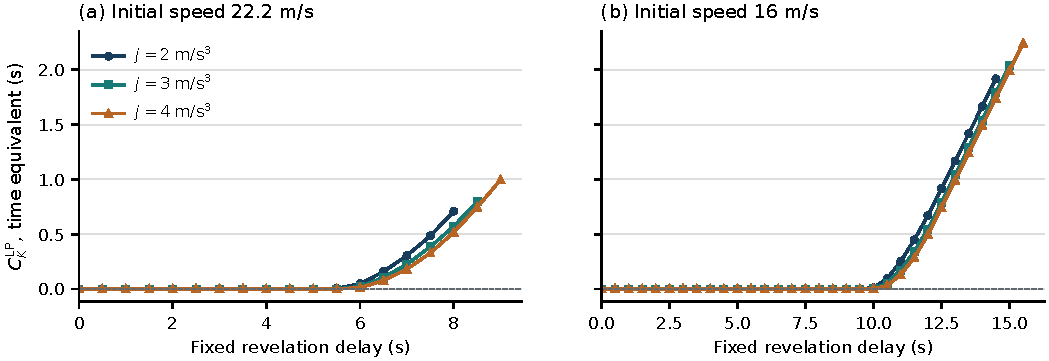
\includegraphics[width=\textwidth]{fig2_lp_reference.pdf}
\renewcommand{\thefigure}{2}
\caption{Optimal lost-progress cost in the sampled LP, plotted against fixed revelation delay. Panels use the two approach speeds; the dashed zero line distinguishes cost-free from costly common preparation. Curves end at the last feasible half-second grid point; the immediately following point is infeasible in every curve. These are model optima, not fitted boundaries of the vehicle experiment.}
\end{figure*}

\subsection{Comparing observed passing costs to the reference}

P-B opens the phase output by position, and actual memory adoption can occur later. For each constant-command passing branch, the measured delay is

\[\Delta_{\rm obs}=t_{\rm info}-t_{200},\tag{18}\]

where \(t_{200}\) is the actual crossing of the 200 m approach boundary. It is not the earlier frozen-state timestamp. Passing-time differences \(\Delta T_{\rm obs}\) use the common 3300 m endpoint and matched early branch, interpolating crossing time within the constant-acceleration substep.

Let \(B_G^{\rm LP}(K)\) denote the passing-branch lost-progress increment of the joint LP optimum, divided by \(v_0\). Choose the lower grid index \(K_-=\lfloor\Delta_{\rm obs}/\delta\rfloor\) and report

\[\Delta T_{\rm obs}=B_G^{\rm LP}(K_-)+R_{\rm ref}.\tag{19}\]

Revealing the scene at the lower grid point relaxes the information restriction. Lemma 2 supplies the within-model ordering of the total optimum. In these computed optima the stopping branch binds \(x_{R,N}=d_0\) and has constant loss, so the ordering also applies to the passing-branch reference. The report retains upper-grid and interpolated values as secondary descriptions; neither is called a lower bound.

\(R_{\rm ref}\) is a signed reference residual, not the within-model rule excess in (17). Vehicle histories, perceived targets, emergency actions, and the 3300 m endpoint differ from the LP assumptions. Its sign is therefore measured, not guaranteed across models.

\section{Experimental Results}

\begin{table*}[!t]
\centering
\renewcommand{\thetable}{II}
\caption{Contributions and their direct evidence. Protocol details are fixed in Table I; the analytical reference and observed vehicle costs remain separate.}
\setlength{\tabcolsep}{3pt}
\renewcommand{\arraystretch}{1.12}
\begin{tabularx}{\textwidth}{@{}>{\hsize=0.600000\hsize\linewidth=\hsize\raggedright\arraybackslash}X>{\hsize=1.020000\hsize\linewidth=\hsize\raggedright\arraybackslash}X>{\hsize=1.380000\hsize\linewidth=\hsize\raggedright\arraybackslash}X@{}}
\toprule
\textbf{Contribution} & \textbf{Direct evidence} & \textbf{Supported result} \\
\midrule
Visual integration & P-V F/S, cue interventions; Tables V and VI & Camera-driven completion, compliance, and localized override contexts \\
Comfort execution & Algorithm 1; P-C, record accounting and memory replay & Complete-executor smoothness effect; distinct propagation and target-update mechanisms \\
Preparation analysis & P-LP and P-B; Fig. 2 and Table VII & Model feasibility/cost separation and observed rule-dependent passing costs \\
\bottomrule\end{tabularx}
\end{table*}

\subsection{Complete execution improves realized smoothness}

Actors A/B share a seed-7 initialization and 40000 actor-frozen adaptation steps, followed by 300000 integration steps with \(\lambda_c=0\) and 0.1, respectively. Their final models are frozen for the P-C executor comparison; both layers include terminal settling. The complete layer combines release and target checks, signal handling, expanded executor access to phase timing, and road-limit enforcement. Freezing the actor does not make this an equal-information or individual-feature ablation.

\begin{table*}[!t]
\centering
\renewcommand{\thetable}{III}
\caption{Fixed-actor complete-executor comparison. Each row contains the same nine completed development trips, including terminal settling. Peak jerk is the maximum; A/B are variants from one training seed. The full configuration includes changed executor information access and road-limit handling. Units: \(I_j\) in m\(^2\)/s\(^5\), jerk in m/s\(^3\), time in s, energy in Wh.}
\setlength{\tabcolsep}{3pt}
\renewcommand{\arraystretch}{1.12}
\begin{tabularx}{\textwidth}{@{}>{\hsize=1.554930\hsize\linewidth=\hsize\raggedright\arraybackslash}X>{\hsize=0.845070\hsize\linewidth=\hsize\centering\arraybackslash}X>{\hsize=0.845070\hsize\linewidth=\hsize\centering\arraybackslash}X>{\hsize=0.883099\hsize\linewidth=\hsize\centering\arraybackslash}X>{\hsize=1.026761\hsize\linewidth=\hsize\centering\arraybackslash}X>{\hsize=0.845070\hsize\linewidth=\hsize\raggedleft\arraybackslash}X@{}}
\toprule
\textbf{Actor / executor} & \textbf{Mean \(I_j\)} & \textbf{Peak jerk} & \textbf{Mean time} & \textbf{Mean energy} & \textbf{Settled} \\
\midrule
A / original & 86.776 & 6.483 & 270.889 & 450.821 & 9/9 \\
A / complete & 63.781 & 2.000 & 271.000 & 446.432 & 9/9 \\
B / original & 60.690 & 6.809 & 303.167 & 363.387 & 9/9 \\
B / complete & 34.249 & 2.000 & 303.556 & 360.970 & 9/9 \\
\bottomrule\end{tabularx}
\end{table*}

For A, mean \(I_j\) falls by \textbf{26.50\%}, with \textbf{0.11 s} extra mean time and \textbf{0.97\%} lower energy. Every condition improves in \(I_j\), by 17.60--36.63\%. B improves by 43.57\% but retains its slower learned pace. The complete executor finishes 18/18 trips without observed signal, local-speed, physical-bound, or fallback events. Removing the terminal-settling tail still reduces A's mean \(I_j\) from 77.861 to 61.879, or 20.53\%; the gain is not solely a settling-window effect. These results measure the full-layer development effect.

The soft regularizer alone had reduced \(I_j\) by 36.96\% under its original arrival cut, while increasing mean time by 11.88\% and failing to reduce worst jerk. Its intervention and endpoint differ from Table III, so the percentages are not additive. Supplementary Section F reports all conditions, development configurations, and their failures. The practical result is that smoothing the preference and preserving a feasible release solve different parts of execution.

\subsection{Timing can preserve an earlier stopping opportunity}

P-T freezes actor A and changes only the executor's use of remaining phase time. Both executors see current color within 1000 m; the actor retains SPaT in both arms.

\begin{table}[!t]
\centering
\renewcommand{\thetable}{IV}
\caption{Executor timing-use comparison. All nine attempted conditions are retained; no incomplete trip is used as a matched complete-route cost.}
\setlength{\tabcolsep}{3pt}
\renewcommand{\arraystretch}{1.12}
\begin{tabularx}{\columnwidth}{@{}>{\hsize=1.253968\hsize\linewidth=\hsize\raggedright\arraybackslash}X>{\hsize=0.765079\hsize\linewidth=\hsize\centering\arraybackslash}X>{\hsize=0.980952\hsize\linewidth=\hsize\raggedleft\arraybackslash}X@{}}
\toprule
\textbf{Outcome} & \textbf{Current color} & \textbf{Color plus timing} \\
\midrule
Settled trips & 8/9 & 9/9 \\
Signal violations & 1 & 0 \\
Fallback substeps & 4 & 0 \\
Peak jerk, m/s\(^3\) & 7.738 & 2.000 \\
\bottomrule\end{tabularx}
\end{table}

Eight pairs have identical trajectories. In condition 7, timing changes acceleration from 0.408 to 0.160 m/s\(^2\) at 177.5 s, 85.87 m before the line, with 2.5 s of green remaining. Subsequent braking permits a stop 2 m before the line and eventual completion. The current-color executor reaches the phase change with 33.98 m remaining at 21.221 m/s; even instantaneous maximum braking would require 64.33 m.

\begin{figure*}[!t]
\centering
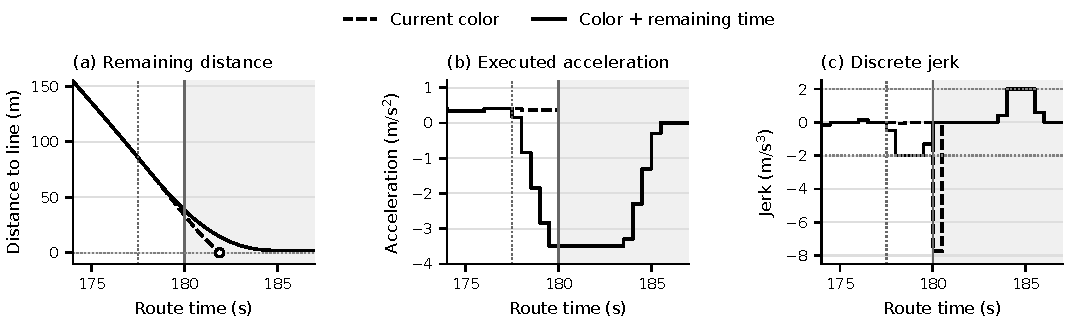
\includegraphics[width=\textwidth]{fig3_timing.pdf}
\renewcommand{\thefigure}{3}
\caption{Matched condition-7 trajectories. Dotted lines mark the first action difference and shading the nonpassable phase. The timing-informed execution changes before stopping becomes unavailable; the other eight paired trajectories are identical. This is an executor timing-use intervention with SPaT available to the actor in both arms.}
\end{figure*}

This identifies one useful preparation opportunity. It neither measures the optimal delay penalty nor supplies a condition-averaged complete-trip gain: the eight jointly completed pairs have zero differences.

\subsection{Camera-driven operation and the learning increment}

\begin{table*}[!t]
\centering
\renewcommand{\thetable}{V}
\caption{Current visual evaluations and a historical probe. Mean R and counts use all attempts. Time, energy, and \(I_j\) means use 24 completed F trips or 27 S trips. The probe's matching identity is incomplete; its nine records are a descriptive reference, not another P-V arm.}
\setlength{\tabcolsep}{3pt}
\renewcommand{\arraystretch}{1.12}
\begin{tabularx}{\textwidth}{@{}>{\hsize=1.644302\hsize\linewidth=\hsize\raggedright\arraybackslash}X>{\hsize=0.681576\hsize\linewidth=\hsize\centering\arraybackslash}X>{\hsize=1.669862\hsize\linewidth=\hsize\centering\arraybackslash}X>{\hsize=0.681576\hsize\linewidth=\hsize\centering\arraybackslash}X>{\hsize=0.681576\hsize\linewidth=\hsize\centering\arraybackslash}X>{\hsize=0.775293\hsize\linewidth=\hsize\centering\arraybackslash}X>{\hsize=0.681576\hsize\linewidth=\hsize\centering\arraybackslash}X>{\hsize=1.184239\hsize\linewidth=\hsize\raggedleft\arraybackslash}X@{}}
\toprule
\textbf{Configuration} & \textbf{Settled} & \textbf{Signal / curve violations} & \textbf{Mean R} & \textbf{Time, s} & \textbf{Energy, Wh} & \textbf{\(I_j\)} & \textbf{Override episodes} \\
\midrule
F, P-V & 24/27 & 2 / 0 & -42.780 & 225.771 & 625.824 & 96.311 & 12/27 \\
S, P-V & 27/27 & 0 / 0 & -39.423 & 223.722 & 597.914 & 88.135 & 9/27 \\
Constant \(u=1\), historical & 9/9 & Not aligned & -39.246 & 217.889 & 605.974 & 100.954 & Not aligned \\
\bottomrule\end{tabularx}
\end{table*}

S completes 27/27 evaluations without a recorded signal or curve-speed violation; 18/27 also avoid jerk overrides. This is an episode-level execution count, not a measure of successful anticipation. Table VI locates the first override in each affected S episode. F's peak jerk of 12.144 m/s\(^3\) occurs near the signal with a nonpassable color estimate during true green; S's peak of 10 m/s\(^3\) occurs at 1.5 m/s in signal-terminal stopping (Supplementary Section G.5).

The constant-command probe shows that perception and execution can themselves support the task. Relative to its archived means, S uses about 1.33\% less energy and 12.70\% less squared jerk, takes 2.68\% longer, and has reward lower by 0.177. The differing protocol identity prevents a causal ranking. These numbers do not establish RL reward superiority. On jointly successful S/F conditions, seed-wise \(I_j\) differences are -12.24, -6.10, and +4.14 with denominators 9, 9, and 6; there is no uniform representation-update comfort benefit.

Cue removal produces the expected functional failures in the archived probes: hiding the curve warning causes overspeed, removing lamp color causes failures, and hiding the endpoint prevents completion. These interventions affect both image paths, so they establish dependence of the complete system on visual cues rather than the isolated contribution of \(Z\). Supplementary Sections B.4 and G give the J/JH gradient routes and separate-protocol outcomes.

Memory contributes both continuity and failure modes. It can retain an earlier green despite a close-range red observation; prolonged detection loss can remove a stopping target. Accepting green assigns an assumed 30 s remaining duration, not an observed countdown. The 200 m rendering range is therefore neither a guaranteed recognition distance nor a guarantee of timely preparation.

\begin{table*}[!t]
\centering
\renewcommand{\thetable}{VI}
\caption{First jerk override in the nine affected S episodes. Categories refer to location and logged context; each episode appears once. The three signal-terminal first events occur at 5.3--5.8 m/s and are not the P-B below-5 m/s classification.}
\setlength{\tabcolsep}{3pt}
\renewcommand{\arraystretch}{1.12}
\begin{tabularx}{\textwidth}{@{}>{\hsize=0.763844\hsize\linewidth=\hsize\raggedright\arraybackslash}X>{\hsize=0.325733\hsize\linewidth=\hsize\centering\arraybackslash}X>{\hsize=1.198697\hsize\linewidth=\hsize\centering\arraybackslash}X>{\hsize=1.711726\hsize\linewidth=\hsize\raggedleft\arraybackslash}X@{}}
\toprule
\textbf{Context} & \textbf{Episodes} & \textbf{Recorded location or state} & \textbf{Interpretation} \\
\midrule
Endpoint handling & 3 & 3986--3993 m; 13--14 m/s & Execution targets extend to 4040--4056 m \\
Near-line color error & 2 & 11--12 m before line; 22.2 m/s & Perceived red/yellow during true green \\
Range update & 1 & About 90 m before line; 13.7 m/s & Distance revision and a positive policy command \\
Signal-terminal stop & 3 & 13--15 m before line & Buffered-target update and stopping \\
\bottomrule\end{tabularx}
\end{table*}

Endpoint targets include a 15 m rule offset. The near-line errors share a camera condition and time across two seeds; the 8 m phase freeze is not yet active at about 11 m. Both trigger braking without a recorded violation. These failures do not establish late first recognition.

\subsection{Preparation rules trade stopping response against passing cost}

P-B comprises 408 branches at 22.2 m/s and 456 at 16 m/s. Each speed combines stop/pass scenes, jerk 2/3/4, a constant command and three frozen S policies, and early or delayed phase output. Feasibility-triggered preparation retains the stopping-backup check; conservative preparation additionally applies a target-speed envelope. The former is labeled min in the archive, without a minimum-cost guarantee. There are eight delayed-distance settings at high speed and nine at low speed.

All 864 branches complete without recorded signal violations; 200 contain emergency jerk overrides, with peak 12.2 m/s\(^3\). The constant-command subset is shown below.

\begin{table*}[!t]
\centering
\renewcommand{\thetable}{VII}
\caption{Constant-command short branches. R denotes stopping. The full approach ends at first stop or line crossing. Passing-time differences use the common 3300 m endpoint and matched early reference; ranges span tested distances and jerk limits.}
\setlength{\tabcolsep}{3pt}
\renewcommand{\arraystretch}{1.12}
\begin{tabularx}{\textwidth}{@{}>{\hsize=0.752456\hsize\linewidth=\hsize\raggedright\arraybackslash}X>{\hsize=1.208251\hsize\linewidth=\hsize\centering\arraybackslash}X>{\hsize=1.074656\hsize\linewidth=\hsize\centering\arraybackslash}X>{\hsize=0.550098\hsize\linewidth=\hsize\centering\arraybackslash}X>{\hsize=1.414538\hsize\linewidth=\hsize\raggedleft\arraybackslash}X@{}}
\toprule
\textbf{Initial speed} & \textbf{Preparation} & \textbf{R: no fallback/override} & \textbf{R branches} & \textbf{Passing \(\Delta T\) range, s} \\
\midrule
22.2 m/s & Early & 2 & 3 & 0.000 to 0.000 \\
22.2 m/s & Feasibility-triggered & 5 & 24 & 0.000 to 1.447 \\
22.2 m/s & Conservative & 16 & 24 & 0.180 to 3.173 \\
16 m/s & Early & 3 & 3 & 0.000 to 0.000 \\
16 m/s & Feasibility-triggered & 14 & 27 & 0.000 to 2.309 \\
16 m/s & Conservative & 27 & 27 & 0.000 to 1.383 \\
\bottomrule\end{tabularx}
\end{table*}

At 22.2 m/s, conservative preparation improves the no-fallback/no-override stopping count but pays 0.180--3.173 s on passing branches. At 16 m/s, some early conservative settings remain cost-free. These are rule-dependent responses, with the assessment windows specified in Supplementary Section H.3.

Geometry remains available during output gating, and acceleration differs before adoption in 55/102 delayed constant-command pairs. S also receives colored pixels. Thus the study measures rule behavior, not a matched-information optimum or one-grid agreement with LP boundaries.

\subsection{Trigger-aligned diagnosis and bounded memory replay}

\begin{table*}[!t]
\centering
\renewcommand{\thetable}{VIII}
\caption{Buffered stopping-target margins and first-event timing. P-B stopping branches; distances in metres. Below-5 m counts include negative margins. Later counts select the first event strictly after adoption. The last column instead locates each branch's first approach event before/at/after adoption or records none.}
\setlength{\tabcolsep}{3pt}
\renewcommand{\arraystretch}{1.12}
\begin{tabularx}{\textwidth}{@{}>{\hsize=1.057320\hsize\linewidth=\hsize\raggedright\arraybackslash}X>{\hsize=0.650658\hsize\linewidth=\hsize\centering\arraybackslash}X>{\hsize=1.382649\hsize\linewidth=\hsize\centering\arraybackslash}X>{\hsize=0.650658\hsize\linewidth=\hsize\centering\arraybackslash}X>{\hsize=0.650658\hsize\linewidth=\hsize\centering\arraybackslash}X>{\hsize=0.769946\hsize\linewidth=\hsize\centering\arraybackslash}X>{\hsize=1.838110\hsize\linewidth=\hsize\raggedleft\arraybackslash}X@{}}
\toprule
\textbf{Initial speed} & \textbf{N} & \textbf{Target-margin range} & \textbf{Negative} & \textbf{Below 5 m} & \textbf{Later events} & \textbf{First: before/at/after/none} \\
\midrule
22.2 m/s & 204 & -1.59--84.08 & 12 & 25 & 111 & 6/6/101/91 \\
16 m/s & 228 & -7.11--123.53 & 19 & 28 & 84 & 0/11/73/144 \\
\bottomrule\end{tabularx}
\end{table*}

All 432 unbuffered line margins are positive, but 408 branches already have stopping targets before adoption. Earlier checks and buffering strongly shape this positivity; it is not independent evidence of timely recognition. The actual target margin is negative in 31 branches, all min, and below 5 m in 53. The first approach event occurs before or at adoption in 23 branches, also all min, while the unknown-color stopping target is active.

The 195 post-adoption diagnostic branches contain 31 adoption-negative, 40 other higher-speed, and 124 terminal cases. Trigger-aligned accounting splits the last group into 92 distance-freeze crossings and 32 creeping cases. In all 92, a fused estimate crosses 15 m before near-line freezing takes effect; 70 have a jerk override. In the 32 creeping cases, the small innovation is fully accounted for by \(e^{\rm prop}\), and none exceeds its jerk bound. They remain fallback diagnostics but are not counted as comfort failures. Supplementary Table S16 preserves all subclasses and timestamps.

At the selected inward update, (13) converts a nonnegative propagated margin to a negative target margin in 191/195 cases: the 32 creeping cases plus 159/163 noncreeping cases. The other four already have negative propagated margin. Its maximum numerical residual is \(1.34\times10^{-14}\) m. In the 31 adoption-negative branches, 15 first become negative at adoption and 16 earlier; a later selected event can be a repeated fallback. The original terminal-event counts, 109/324 for S and 15/108 for the constant policy, therefore combine two mechanisms. Higher-speed counts are 46/324 and 25/108.

At every selected post-adoption event's preceding state, only the buffered target excludes the tested backup: substituting the estimated or true unbuffered line restores a candidate interval in 195/195. This isolates a local target effect without evaluating buffer removal during driving. The three P-V signal-terminal contexts also involve range-memory behavior, but cannot be assumed to share one sufficient repair.

To test the proposed interface change without retraining, complete memory replay uses all 27 S detection streams and their fixed recorded motion. Original memory is reproduced at 12,081 timestamps with zero mismatches. The displacement-consistent guard restores the static buffered backup margin in two of three selected P-V terminal states; one remains negative. Recursive replay also changes two phase-memory records because the revised range postpones existing passed-line track clearing. The two positive margins describe selected recorded states; complete P-B memory replay is unavailable. The guard remains experimental because fixed motion omits the feedback of changed actions on later observations and target estimates.

All floor-reference residuals in (19) remain nonnegative for the 102 constant-command passing branches: 0--0.837 s and 0.180--2.225 s for high-speed min and conservative preparation; 0--2.117 s and 0--1.309 s at 16 m/s. The 8.106 s case has a feasible 8.0 s floor but infeasible 8.5 s upper value. Upper-grid or interpolated quantities are secondary references, with the cross-model limits stated in Section V-C.

\subsection{Structured 20 km reference context}

The eight structured-input 20 km seeds each retain 5 million integration steps, twenty checkpoints, six selection conditions, and six reporting conditions within the development grid. The best selected seed has reference-relative regret 6.43 versus the attentive driver's 10.41. Five selected seeds outperform the 18.5 m/s rule, but only two do so on late means. Across seeds, selected return is -177.37 (sample SD 3.31) and late return -183.15 (between-seed SD 5.75), versus -177.29 for the rule.

A typical long-route advantage is not established. Supplementary Section I reports all seeds and unfinished outcomes; their energy-time residual differs from the preparation penalty in (16).

\section{Discussion}

Target formation, command realization, and preparation cost connect the contributions. The strongest measured effect is the complete executor's smoothness improvement. Camera-based completion establishes operation, without demonstrating RL superiority over the historical constant-command probe.

The record audit identifies a concrete interface requirement: motion prediction and target revision must use consistent displacement, and a distance-freeze rule must inspect the candidate update that can exhaust a retained response. The reserve after projection can be smaller than the next inward revision. This explains why an earlier stop target does not automatically make execution robust. The bounded guard replay is also informative: a local repair can alter later phase memory and leave another negative margin unresolved. A target-update method must therefore be assessed recursively, with remaining failure cases retained.

Scope remains the synthetic development routes. Shared visual data, unequal protocol information, archived critic semantics, assumed green duration, and emergency overrides limit inference. The companion enables interface reuse; it does not establish real-road generalization.

\section{Conclusion}

Camera-derived targets, reinforcement learning commands, release-aware execution, and an LP preparation reference support a concrete longitudinal driving system. Its visual configuration completes 27/27 development evaluations without recorded signal or curve-speed violations; a separate complete-executor comparison reduces squared jerk by 26.50\% with 0.11 s extra mean time.

Trigger-aligned records show how small propagation discrepancies and larger target revisions produce different fallback mechanisms. Full memory replay reproduces the recorded outputs of the original update chain and characterizes an experimental guard at selected fixed-motion states. Together with the locally installable environment, the results make target quality, actual motion, and preparation cost reproducible engineering objects with explicit limits on training semantics, information access, and fixed-motion replay.
\begin{thebibliography}{99}
\bibitem{R-DP1} H. Yang, F. Almutairi, and H. Rakha, ``Eco-driving at signalized intersections: a multiple signal optimization approach,'' \emph{IEEE Trans. Intell. Transp. Syst.}, vol.~22, no. 5, pp.~2943--2955, May 2021, doi: 10.1109/TITS.2020.2978184.
\bibitem{R-DP2} A. Hamednia, N. K. Sharma, N. Murgovski, and J. Fredriksson, ``Computationally efficient algorithm for eco-driving over long look-ahead horizons,'' \emph{IEEE Trans. Intell. Transp. Syst.}, vol.~23, no. 7, pp.~6556--6570, Jul.~2022, doi: 10.1109/TITS.2021.3058418.
\bibitem{R-CURV} J. Liu, W. Zhuang, Y. Ding, L. Wang, H. Chen, and C.-A. Tan, ``Energy-oriented speed profile optimization for electric vehicles considering road horizontal curvature,'' \emph{J. Braz. Soc. Mech. Sci. Eng.}, vol.~44, no. 10, art. 453, 2022, doi: 10.1007/s40430-022-03723-4.
\bibitem{R-RL1} J. Li, A. Fotouhi, W. Pan, Y. Liu, Y. Zhang, and Z. Chen, ``Deep reinforcement learning-based eco-driving control for connected electric vehicles at signalized intersections considering traffic uncertainties,'' \emph{Energy}, vol.~279, art. 128139, Sep.~2023, doi: 10.1016/j.energy.2023.128139.
\bibitem{R-RL2} J. Li, Y. Wang, H. He, H. Wang, and X. Meng, ``Safe reinforcement learning-based eco-driving strategy for connected electric vehicles at signalized intersection,'' \emph{Automotive Innovation}, vol.~8, no. 4, pp.~998--1014, 2025, doi: 10.1007/s42154-025-00362-y.
\bibitem{R-RL3} Z. Bai, P. Hao, W. ShangGuan, B. Cai, and M. J. Barth, ``Hybrid reinforcement learning-based eco-driving strategy for connected and automated vehicles at signalized intersections,'' \emph{IEEE Trans. Intell. Transp. Syst.}, vol.~23, no. 9, pp.~15850--15863, Sep.~2022, doi: 10.1109/TITS.2022.3145798.
\bibitem{R-IZOO} V. Jayawardana, B. Freydt, A. Qu, C. Hickert, Z. Yan, and C. Wu, ``IntersectionZoo: Eco-driving for benchmarking multi-agent contextual reinforcement learning,'' arXiv:2410.15221, 2024, https://arxiv.org/abs/2410.15221.
\bibitem{R-TD3} S. Fujimoto, H. van Hoof, and D. Meger, ``Addressing function approximation error in actor-critic methods,'' in \emph{Proc. 35th Int. Conf. Machine Learning (ICML)}, 2018, pp.~1587--1596.
\bibitem{R-CAPS} S. Mysore, B. Mabsout, R. Mancuso, and K. Saenko, ``Regularizing action policies for smooth control with reinforcement learning,'' in \emph{Proc. IEEE Int. Conf. Robotics and Automation (ICRA)}, 2021, arXiv:2012.06644, https://arxiv.org/abs/2012.06644.
\bibitem{R-RUCKIG} L. Berscheid and T. Kröger, ``Jerk-limited real-time trajectory generation with arbitrary target states,'' in \emph{Robotics: Science and Systems}, 2021, doi: 10.15607/RSS.2021.XVII.015, https://arxiv.org/abs/2105.04830.
\bibitem{R-PSF} K. P. Wabersich and M. N. Zeilinger, ``A predictive safety filter for learning-based control of constrained nonlinear dynamical systems,'' \emph{Automatica}, vol.~129, art. 109597, 2021, https://arxiv.org/abs/1812.05506.
\bibitem{R-BCBF} Y. Chen, M. Jankovic, M. Santillo, and A. D. Ames, ``Backup control barrier functions: formulation and comparative study,'' arXiv:2104.11332, 2021, https://arxiv.org/abs/2104.11332.
\bibitem{R-PROJ} H. Markgraf, S. Sawant, H. Krasowski, L. Schäfer, S. Gros, and M. Althoff, ``Safe reinforcement learning using action projection: safeguard the policy or the environment?'' arXiv:2509.12833, 2025, https://arxiv.org/abs/2509.12833.
\bibitem{R-ASR} B. Huang, C. Lu, L. Leqi, J. M. Hernández-Lobato, C. Glymour, B. Schölkopf, and K. Zhang, ``Action-sufficient state representation learning for control with structural constraints,'' in \emph{Proc. 39th Int. Conf. Machine Learning (ICML)}, vol.~162, 2022, pp.~9260--9279, https://proceedings.mlr.press/v162/huang22f.html.
\bibitem{R-VE} D. Arumugam and B. Van Roy, ``Deciding what to model: value-equivalent sampling for reinforcement learning,'' arXiv:2206.02072, 2022, https://arxiv.org/abs/2206.02072.
\bibitem{R-PREVIEW} P. Seiler, A. A. Ozdemir, and G. J. Balas, ``Performance limits with preview information and actuator rate constraints,'' in \emph{Proc. American Control Conference}, 2012, pp.~5532--5537, doi: 10.1109/ACC.2012.6314725.
\bibitem{S4} ``2019 Nissan Leaf Plus benchmarking,'' NHTSA docket NHTSA-2023-0022-0017, attachment 47, 2023.
\bibitem{S3} A. Nikolian \emph{et al.}, ``Lithium-ion batteries---development of advanced electrical equivalent circuit models for nickel manganese cobalt lithium-ion,'' \emph{Energies}, vol.~9, no. 5, art. 360, 2016, doi: 10.3390/en9050360.
\bibitem{S5} Idaho National Laboratory, Advanced Vehicle Testing Activity, battery pack test reports, 2011 and 2013 Nissan Leaf.
\end{thebibliography}
\begin{IEEEbiographynophoto}{Ziran Peng}is with the School of Transportation and Electrical Engineering, Hunan University of Technology, Zhuzhou, China.\end{IEEEbiographynophoto}
\begin{IEEEbiographynophoto}{Zeyu Fan}is with the School of Transportation and Electrical Engineering, Hunan University of Technology, Zhuzhou, China.\end{IEEEbiographynophoto}

\end{document}
